\documentclass[a4paper,notitlepage]{article}

\usepackage{fullpage}
\usepackage{graphicx}
\usepackage{float}
\usepackage{appendix}
\usepackage{listings}
\usepackage{xcolor}

\definecolor{mGreen}{rgb}{0,0.6,0}
\definecolor{mGray}{rgb}{0.5,0.5,0.5}
\definecolor{mPurple}{rgb}{0.58,0,0.82}
\definecolor{backgroundColour}{rgb}{0.95,0.95,0.92}

\lstdefinestyle{CStyle}{
    backgroundcolor=\color{backgroundColour},
    commentstyle=\color{mGreen},
    keywordstyle=\color{magenta},
    numberstyle=\tiny\color{mGray},
    stringstyle=\color{mPurple},
    basicstyle=\footnotesize,
    breakatwhitespace=false,
    breaklines=true,
    captionpos=b,
    keepspaces=true,
    numbers=left,
    numbersep=5pt,
    showspaces=false,
    showstringspaces=false,
    showtabs=false,
    tabsize=2,
    language=C
}

\renewcommand{\contentsname}{Contenidos}

\begin{document}
\tableofcontents
\section{Resolución}
El árbol AVL implementado se basa en la estructura avltree{\_}t, la cual puede
representar un nodo de un árbol o un árbol completo según cómo se lo interprete
(root en la función main es el nodo raíz del árbol, pero también representa al
árbol completo). Esta estructura contiene dos punteros a otros objetos de su
mismo tipo que representan la rama izquierda y derecha del nodo, un entero que
representa el valor almacenado y un entero no signado para almacenar la altura
del nodo en el árbol.

Se implementaron una serie de funciones para interactuar con punteros a
avltree{\_}t de modo que un usuario de la estructura no necesite acceder a los
miembros de forma directa. También se implementaron algunas funciones con
declaraciones un poco más específicas para resoluciones de problemas
particulares, no se espera que un usuario utilice estas funciones. Con esa
distinción, la lista de funciones públicas es la siguiente:

\begin{itemize}
    \item avltree{\_}new{\_}node
    \item avltree{\_}free
    \item avltree{\_}search
    \item avltree{\_}insert
    \item avltree{\_}delete
    \item avltree{\_}print
    \item avltree{\_}get{\_}balance{\_}factor
    \item avltree{\_}get{\_}height
\end{itemize}

Los métodos "privados" que no deberían ser utilizados por usuarios directamente
son los siguientes:

\begin{itemize}
    \item avltree{\_}pop{\_}leaf
    \item avltree{\_}replace{\_}node
    \item avltree{\_}delete{\_}inner
    \item avltree{\_}print{\_}inner
    \item avltree{\_}rotate
    \item avltree{\_}balance
    \item avltree{\_}insert{\_}inner
\end{itemize}

En un proyecto más real, avltree{\_}t y sus funciones vivirían en un archivo .c
y sólo se expondrían las funciones públicas mediante un .h, por simplicidad
aquí se decidió dejar todo en un mismo archivo fuente.

La documentación para cada función está en el código en formato doxygen.

\pagebreak

\section{Preguntas}
\subsection{Crear un árbol binario de la siguiente forma.}
\begin{figure}[H]
    \centering
    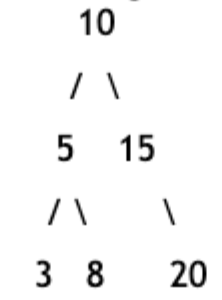
\includegraphics[scale=0.65]{imgs/base-tree.png}
\end{figure}

Para representar el árbol, se eligió un formato distinto en el que los nodos
se imprimen en una forma similar al comando tree. Se puede ver comparando las
representaciones que el subnodo superior en esta representación corresponde
al lado izquierdo del nodo y el inferior al derecho. Las ramas que no apuntan
a un nodo sólo imprimen la flecha sin un número asociado. Las hojas del árbol
no imprimen ninguna flecha para que sea más fácil la visualización.

\begin{figure}[H]
    \centering
    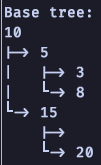
\includegraphics[scale=0.65]{imgs/base-tree-run.png}
\end{figure}

\subsection{Implementar el método “insertar nodo” e insertar el nodo 24.}
Tras insertar el nuevo nodo, este desbalancea el árbol hacia la derecha del nodo
20 y provoca una rotación DD, con el siguiente resultado:

\begin{figure}[H]
    \centering
    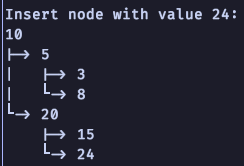
\includegraphics[scale=0.65]{imgs/insert-node.png}
\end{figure}

\pagebreak

\subsection{Implementar el método “eliminar nodo” y eliminar el nodo 20.}
Se elimina el nodo 20, el árbol permanece balanceado:

\begin{figure}[H]
    \centering
    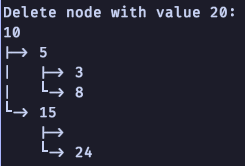
\includegraphics[scale=0.65]{imgs/delete-node.png}
\end{figure}

\subsection{Implementar el método “buscar nodo”.}
El método se implementó y a modo de prueba se lo utilizó para imprimir el árbol
a partir del nodo 5

\begin{figure}[H]
    \centering
    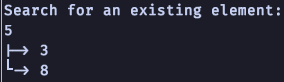
\includegraphics[scale=0.65]{imgs/search.png}
\end{figure}

\subsection{Implementar los métodos de rotación.}
Se implementó un único método de rotación avltree{\_}rotate que toma el sentido
de rotación deseado y realiza rotaciones simples. Para rotaciones dobles, la
función avltree{\_}balance se encarga de determinar las rotaciones necesarias
en base a los factores de equilibrio de los nodos participantes y realizar
multiples llamados a avltree{\_}rotate de forma acorde.

\subsection{¿Cuál es el factor de equilibrio del nodo con valor 10?}
El nodo 10 tiene un factor de equilibrio de 0, ya que sus ramas tienen la misma
altura.

\subsection{¿Cuál es la altura del árbol AVL?}
El árbol AVL posee una altura de 3.

\begin{appendix}
    \section{Código utilizado}
    \lstinputlisting[style=CStyle]{../src/main.c}
\end{appendix}
\end{document}
